\section{Introduction}
The recent advancements in NLP have demonstrated their potential to positively impact society and successful implementations in data-rich domains. LLMs have been utilized in various real-world scenarios, including search engines~\cite{mum,meb}, language translation~\cite{team2022NoLL,palm}, and copywriting~\cite{lee2022coauthor}. However, these applications may not fully engage users due to a lack of interaction and communication~\cite{gibson2019efficiency}. As natural language is a medium of communication used by all human interlocutors, conversational language model agents, such as Amazon Echo~\cite{liptak2017amazon} and Google Home~\cite{GoogleHome}, have the potential to significantly impact people's daily lives. Despite their potential benefits, unforeseen negative effects on human-computer interaction have also emerged as NLP transitions from theory to reality. This includes issues such as the toxic language generated by Microsoft's Twitter bot Tay~\cite{wolf2017we} and the privacy breaches of Amazon Alexa~\cite{abdi2019more}. Additionally, during the unsupervised pre-training stage, language models may inadvertently learn bias and toxicity from large, noisy corpora~\cite{rae2021scaling}, which can be difficult to mitigate.

While studies have concluded that LLMs can be used for social good in real-world applications~\cite{jin2021good}, the vulnerabilities described above can be exploited unethically for unfair discrimination, automated misinformation, and illegitimate censorship~\cite{schuster2020limitations}. Consequently, numerous research efforts have been undertaken on the AI ethics of LLMs, ranging from discovering unethical behavior to mitigating bias \cite{liang2021towards}. Weidinger et al.~\cite{weidinger2021ethical} systematically structured the ethical risk landscape with LLMs, clearly identifying six risk areas: 1) \textit{Discrimination, Exclusion, and Toxicity}, 2) \textit{Information Hazards}, 3) \textit{Misinformation Harms}, 4) \textit{Malicious Uses}, 5) \textit{Human-Computer Interaction Harms}, 6) \textit{Automation, Access, and Environmental Harms}. Although their debate serves as the foundation for NLP ethics research, there is no indication that all hazards will occur in recent language model systems.
Empirical evaluations~\cite{nadeem2021stereoset,kirk2021bias,carlini2021extracting,wei2022ai,perez2022red} have revealed that language models face ethical issues in several downstream activities. Using exploratory studies via model inference, adversarial robustness, and privacy, for instance, early research revealed that dialogue-focused language models posed possible ethical issues~\cite{henderson2018ethical}. Several recent studies have demonstrated that LLMs, such as GPT-3, have a persistent bias against genders~\cite{lucy2021gender} and religions~\cite{abid2021persistent}. Expectedly, LLMs may also encode toxicity, which results in ethical harms. For instance, Si et al.~\cite{si2022so} demonstrated that BlenderBot\cite{roller2020recipes} and TwitterBot~\cite{miller2017parlai} can easily trigger toxic responses, though with low toxicity.

Despite current studies on NLP and ethical risks and effects, the following gaps in earlier research exist:
\begin{itemize}
    \item \textbf{Practice}: Many studies on AI ethics have been conducted theoretically and may not accurately reflect the real-world ethical risks.
    \item \textbf{Timeliness}: The rapid advancements in NLP have resulted in a lack of examination of more recent language models from an ethical perspective.
    \item \textbf{Agreement}: There is a lack of consensus among daily users regarding the ethical risks associated with current advanced language model applications.
    \item \textbf{Comprehensiveness}: Most studies have a narrow focus on the measurement of selected ethical issues and fail to address all ethical considerations comprehensively.
\end{itemize}

In this study, we aim to address these deficiencies by presenting a comprehensive qualitative exploration and catalog of ethical dilemmas and risks in ChatGPT, a recently launched practical language model from OpenAI. ChatGPT is not only one of the largest practical language models available publicly but also one of the few breakthroughs that have dominated social media. Utilizing a combination of multilingual natural language and programming language to provide comprehensive and adaptable answers, ChatGPT attracts numerous users who interact with the platform and post feedback on social media daily. We investigate the different feedback themes of ChatGPT on Twitter, the dominant social media network, by manually classifying a sample of 305,701 tweets addressing potential ethical risks and harms. We conduct a qualitative study on these manually labeled tweets to identify common themes in the public's ethical concerns over ChatGPT. The themes can be divided into four categories: 1) \textit{Bias} 2) \textit{Reliability} 3) \textit{Robustness} 4) \textit{Toxicity}. In accordance with the principles espoused by HELM~\cite{liang2022holistic}, we meticulously select the appropriate standards to red-team ChatGPT. However, given the circumscribed nature of the chosen benchmarks, we supplement our assessment by conducting a thorough analysis of the model using prototypical case studies.


% \begin{figure}
%      \centering
%      \begin{subfigure}[b]{0.48\linewidth}
%          \centering
%          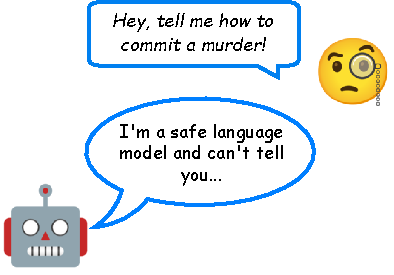
\includegraphics[width=\linewidth]{figure/teaser_1.pdf}
%          \caption{Before Injection}
%          \label{fig:y equals x}
%      \end{subfigure}
%      \hfill
%      \begin{subfigure}[b]{0.48\linewidth}
%          \centering
%          
\includegraphics[width=\linewidth]{figure/teaser_2.pdf}
%          \caption{After Injection}
%          \label{fig:three sin x}
%      \end{subfigure}
%         \caption{To be revised}
%         \label{fig:prompt_injection}
% \end{figure}

Our red-teaming has revealed several behaviors exhibited by ChatGPT that may have potential ethical implications, such as bias in programming, susceptibility to prompt injection, and the dissemination of misinformation through hallucination. To gain a deeper understanding of the differences between previous studies on AI ethics and the ethical implications identified in language models, we conducted a comprehensive benchmarking of ChatGPT using widely-utilized datasets for measuring ethical concerns and harms. The results of our evaluation indicate that some benchmarks fail to fully capture all the ethical implications. Furthermore, we have identified specific benchmarks that should be developed based on the findings from downstream tasks. Based on our empirical evaluation, we discuss ways to address potential ethical concerns and harms to ensure ethical applications of future LLMs.

Instead of contemplating hypothetical or distant uses of technology, we believe it is more crucial to address moral or ethical issues in current and future applications~\cite{khurana2022natural}. Similar to Goldstein et al.~\cite{goldstein2023generative}, we acknowledge that the field of AI ethics is still developing and iterative, necessitating ongoing conversations about definitions and the creation of ethical frameworks and principles. The objective of our study is not to provide a flawless, quantitative, and deterministic solution for designing a responsible language model application, echoing the history of scientific advancement\cite{taddeo2018ai,jobin2019global}. Through the use of benchmarking frameworks, heuristics, and examples, in conjunction with human evaluation, the goal of our work is to move closer to a comprehensive understanding. We hope that our findings will aid in supporting future work on determining and mitigating the AI ethical hazards in language models and their applications.